\twocolumn[\colorsection{Preguntas para el análisis}]
\textit{En esta sección se requiere brindar respuestas argumentadas.}
\setcounter{figure}{0}
%
\begin{Exercise}
    Se coloca una lámina de cobre entre los polos de un electroimán con el campo magnético perpendicular a la lámina. Cuando se tira de la lámina hacia afuera, se requiere una fuerza considerable, la cual aumenta con la rapidez. Explique este fenómeno.
\end{Exercise}
%
\begin{Exercise}\label{p:preguntasIV01}
    En la figura \ref{f:preguntasIV01}, si la rapidez angular $\omega$ de la espira se duplica, entonces la frecuencia con la que la corriente inducida cambia de sentido también se duplica, al igual que la f.e.m máxima. ¿Por qué? ¿Cambia el torque requerido para hacer girar la espira?
\end{Exercise}
%
\begin{center}
  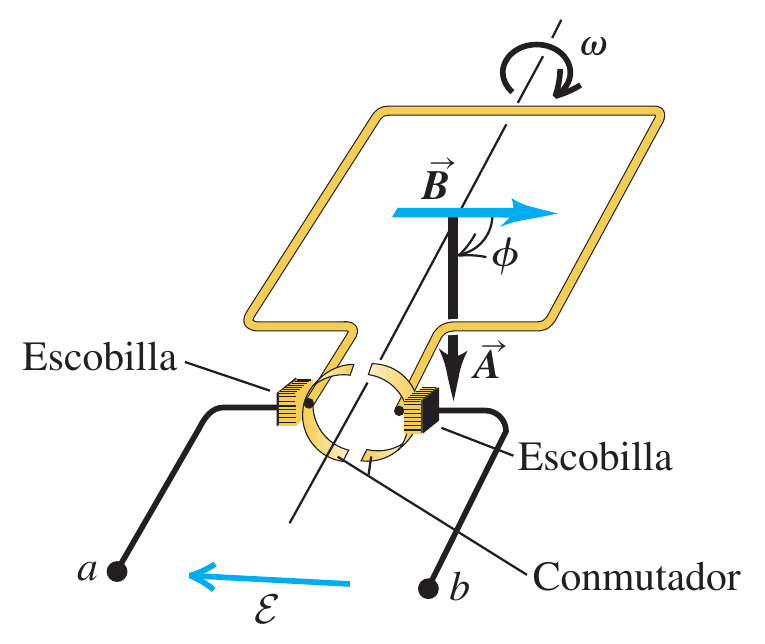
\includegraphics[scale=0.3]{preguntas-01.png}
  \captionof{figure}{Pregunta \ref{p:preguntasIV01}\label{f:preguntasIV01}}
\end{center}
%
\begin{Exercise}
    Dos espiras circulares se encuentran lado a lado en el mismo plano. Una está conectada a una fuente que suministra una corriente creciente; la otra es un anillo cerrado simple. ¿La corriente inducida en el anillo tiene el mismo sentido que la corriente en la espira conectada con la fuente o es opuesto? ¿Qué sucede si disminuye la corriente en la primera espira?
\end{Exercise}
%
\begin{Exercise}
    Un conductor largo y recto pasa por el centro de un anillo metálico, perpendicular a su plano. Si la corriente en el conductor aumenta, ¿se induce una corriente en el anillo?
\end{Exercise}
%
\begin{Exercise}
    Un estudiante asegura que, si se deja caer en forma vertical un imán permanente por un tubo de cobre, finalmente el imán alcanza una velocidad terminal, aunque no haya resistencia del aire. ¿Por qué tendría que ser así?
\end{Exercise}
%
\begin{Exercise}
    Un avión vuela horizontalmente sobre la Antártida, donde el campo magnético terrestre está dirigido mayormente hacia arriba alejándose del suelo. Vista por un pasajero que mira hacia el frente del avión, ¿el extremo del ala izquierda está a un potencial eléctrico mayor que el del ala derecha? ¿La respuesta depende de la dirección en que vuela el avión?
\end{Exercise}
%
\begin{Exercise}
    Un rectángulo de metal está cerca de un alambre largo, recto y que conduce corriente, con dos de sus lados paralelos al alambre. Si la corriente en el alambre está disminuyendo, ¿el rectángulo es repelido o atraído por el alambre? Explique por qué este resultado es congruente con la ley de Lenz.
\end{Exercise}
%
\begin{Exercise}\label{p:preguntasIV02}
    En la situación que se muestra en la figura \ref{f:preguntasIV02}, ¿sería adecuado preguntar cuánta energía gana un electrón durante un recorrido completo alrededor de la espira de alambre con corriente $I$? ¿Sería adecuado preguntar a través de qué diferencia de potencial se mueve el electrón durante ese recorrido completo?
\end{Exercise}
%
\begin{center}
    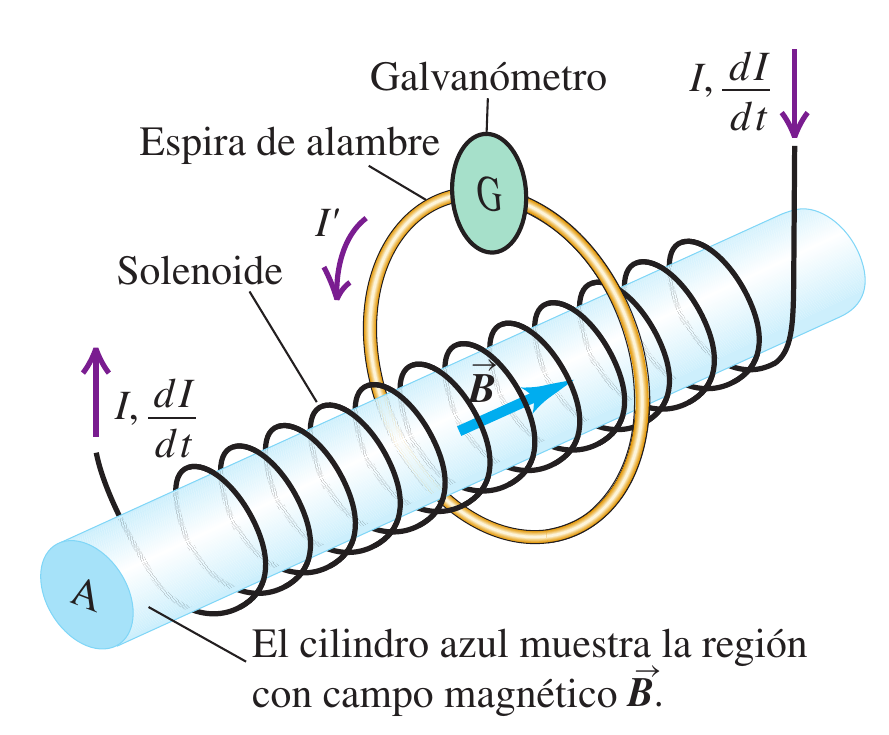
\includegraphics[scale=0.3]{preguntas-02.png}
    \captionof{figure}{Pregunta \ref{p:preguntasIV02}\label{f:preguntasIV02}}
\end{center}
%
\begin{Exercise}
    Una espira conductora cuadrada está en una región de campo magnético constante y uniforme. ¿La espira puede hacerse girar alrededor de un eje a lo largo de un lado sin que se induzca alguna fem en la espira? Explique lo que sucede en términos de la orientación del eje de rotación con respecto a la dirección del campo magnético.
\end{Exercise}
%
\begin{Exercise}
    Indique cuáles de los siguientes enunciados son verdaderos y justifique su elección.
    \begin{itemize}
        \item $\int\int \vec{B} \cdot d\vec{S} = 0 \Leftrightarrow \varepsilon_{ind} = 0$
        \item El signo negativo de la ley de Faraday es consecuencia del principio de acción y reacción.
        \item Un solenoide puede considerarse ideal si es muy largo.
        \item Una corriente variable no puede inducir una fem de valor constante.
        \item $\varepsilon_{ind} \neq 0 \Rightarrow \int\int \vec{B} \cdot d\vec{S} \neq 0$
        \item Una corriente estacionaria genera un campo magnético estacionario y no necesariamente uniforme.
        \item Una bobina almacena energía del campo eléctrico.
        \item La energía almacenada por una bobina es independiente del valor de la corriente que la circula.
        \item Un campo magnético variable siempre induce una f.e.m en toda espira sumergida en él.
        \item El campo magnético inducido es siempre opuesto al campo magnético externo.
        \item El signo negativo en la ley de Faraday-Lenz es consecuencia de la conservación de la energía.
    \end{itemize}
\end{Exercise}
%
\begin{Exercise}
    Para resistencias muy grandes, es fácil construir circuitos $RC$ que tengan constantes de tiempo de varios segundos o minutos. ¿Cómo se utilizaría este hecho para medir resistencias muy grandes, demasiado grandes como para medirlas con métodos más convencionales?
\end{Exercise}
%
\begin{Exercise}
    Cuando un capacitor, una batería y un resistor se conectan en serie, ¿el resistor afecta la carga máxima que se almacena en el capacitor? ¿Por qué? ¿Qué finalidad tiene el resistor?
\end{Exercise}
%
\begin{Exercise}\label{p:preguntasIV03}
    En el circuito mostrado en la figura \ref{f:preguntasIV03}, cuando se cierra el interruptor, el potencial $V_{ab}$ cambia súbitamente y en forma discontinua, a diferencia de la corriente. Explique por qué el voltaje puede cambiar de pronto, pero la corriente no.
\end{Exercise}
%
\begin{center}
\begin{circuitikz}[scale=1]
    \draw (0,1.5) to[R=$R$, color=red] (2.5,1.5) to[L, l=$L$, color=green!80!black] (5,1.5)
    (0,1.5) -- (0,3) to[battery2, color=cyan] (2.5,3) to[switch] (5,3) -- (5,1.5);
    \fill (0,1.5) circle (3pt) node [below] {$a$};
    \fill (2.5,1.5) circle (3pt) node [below] {$b$};
\end{circuitikz}
\captionof{figure}{Pregunta \ref{p:preguntasIV03}\label{f:preguntasIV03}}
\end{center}
%
\begin{Exercise}
    Suponga que hay una corriente estable en un inductor. Si trata de reducir la corriente a cero en forma instantánea abriendo rápidamente un interruptor, puede aparecer un arco donde el interruptor hace contacto. ¿Por qué? ¿Es físicamente posible detener la corriente de forma instantánea? Explique su respuesta.
\end{Exercise}
%